\definecolor{yellowgreen}{RGB}{154,205,50}    
\definecolor{limeyellow}{RGB}{185,215,40}     
\definecolor{yellowgreenyellow}{RGB}{173,255,47}    

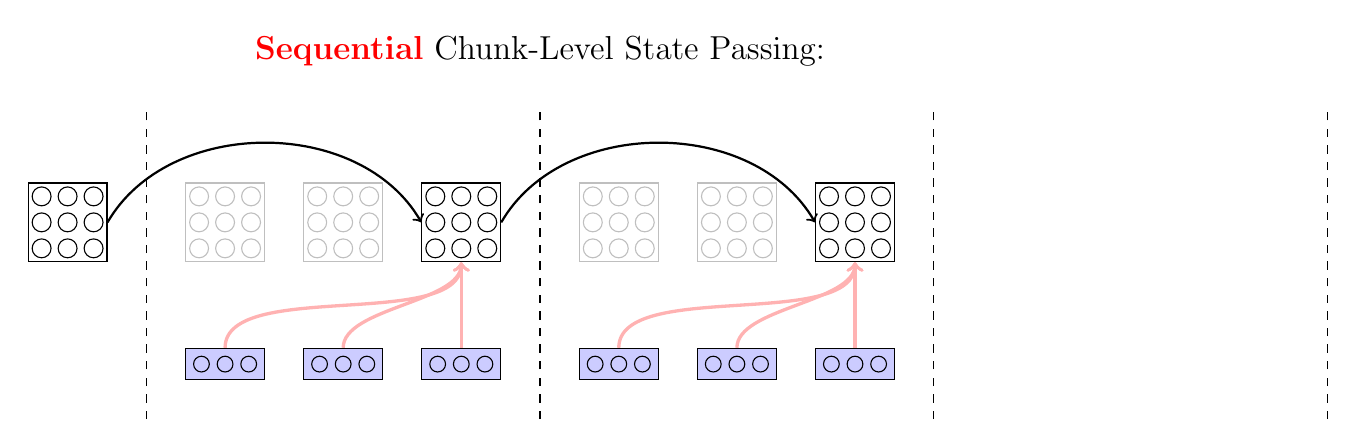
\begin{tikzpicture}
    \foreach \x in {0,5,10,15} {
        \draw[dashed] (\x,-2) -- (\x,2);
    }

        \begin{scope}[shift={(-1.5,0)}]
            \node[draw=black, minimum size=1cm] (grid-0-3) at (0.5,0.5) {};
            \foreach \x in {0,0.33,0.66} {
                \foreach \y in {0,0.33,0.66} {
                    \draw[black] (\x+0.17,\y+0.17) circle (0.12);
                }
            }
        \end{scope}

    \foreach \section [count=\i] in {0.5,5.5} {
        \foreach \offset [count=\j] in {0,1.5} {
            \begin{scope}[shift={(\section+\offset,0)}]
                \node[draw=gray!50, minimum size=1cm] (grid-\i-\j) at (0.5,0.5) {};
                \foreach \x in {0,0.33,0.66} {
                    \foreach \y in {0,0.33,0.66} {
                        \draw[gray!50] (\x+0.17,\y+0.17) circle (0.12);
                    }
                }
            \end{scope}
        }
        
        \begin{scope}[shift={(\section+3,0)}]
            \node[draw=black, minimum size=1cm] (grid-\i-3) at (0.5,0.5) {};
            \foreach \x in {0,0.33,0.66} {
                \foreach \y in {0,0.33,0.66} {
                    \draw[black] (\x+0.17,\y+0.17) circle (0.12);
                }
            }
        \end{scope}
    }
    
    \foreach \section [count=\i] in {0.5,5.5} {
        \begin{scope}[shift={(\section,-1.5)}]
            \foreach \offset [count=\j] in {0,1.5,3} {
                \node[fill=blue!20,draw=black, minimum width=1cm, minimum height=0.4cm] (rect-\i-\j) at (\offset+0.5,0.2) {};
                \foreach \x in {0.2, 0.5, 0.8} {
                    \draw[black] (\offset+\x,0.2) circle (0.1);
                }
                \draw[->,red!30,very thick] (rect-\i-\j.north) to[out=90,in=-90, looseness=0.7] 
                    ([xshift=\j*0cm]grid-\i-3.south);
            }
        \end{scope}
    }
    
% \draw[->,yellowgreen,very thick] (grid-1-3.east) to[bend left=60] node[above,font=\small,xshift=-0.5cm]{$\color{black}\boldsymbol{S}_{[2]}=\boldsymbol{S}_{[1]}{\color{yellowgreen}(\boldsymbol{I}-\boldsymbol{W}_{[2]}^\top \boldsymbol{K}_{[2]})} + {\color{red}\boldsymbol{U}_{[2]}^\top \boldsymbol{K}_{[2]}}$}  (grid-2-3.west);
\draw[->,black, thick] (grid-0-3.east)  to[bend left=60] (grid-1-3.west);
\draw[->,black, thick] (grid-1-3.east)  to[bend left=60] 
node[above,xshift=-1.5cm, yshift=0.5cm,align=center]{
  \textcolor{black}{{\large{\textbf{\color{red}Sequential}} Chunk-Level State Passing:}} \\
%   $\color{black}\boldsymbol{S}_{[i+1]}=\boldsymbol{S}_{[i]}
% + 
%     {\color{blue!50}\colorbox{red!30}{$\boldsymbol{V}_{[i]}^\top \boldsymbol{K}_{[i]}$}}$
} (grid-2-3.west);


\end{tikzpicture}
